% Options for packages loaded elsewhere
\PassOptionsToPackage{unicode}{hyperref}
\PassOptionsToPackage{hyphens}{url}
\PassOptionsToPackage{dvipsnames,svgnames,x11names}{xcolor}
\documentclass[
  french,
  11pt,
  a4paper,
]{article}
\usepackage{xcolor}
\usepackage[margin=2.2cm]{geometry}
\usepackage{amsmath,amssymb}
\setcounter{secnumdepth}{-\maxdimen} % remove section numbering
\usepackage{iftex}
\ifPDFTeX
  \usepackage[T1]{fontenc}
  \usepackage[utf8]{inputenc}
  \usepackage{textcomp} % provide euro and other symbols
\else % if luatex or xetex
  \usepackage{unicode-math} % this also loads fontspec
  \defaultfontfeatures{Scale=MatchLowercase}
  \defaultfontfeatures[\rmfamily]{Ligatures=TeX,Scale=1}
\fi
\usepackage{lmodern}
\ifPDFTeX\else
  % xetex/luatex font selection
\fi
% Use upquote if available, for straight quotes in verbatim environments
\IfFileExists{upquote.sty}{\usepackage{upquote}}{}
\IfFileExists{microtype.sty}{% use microtype if available
  \usepackage[]{microtype}
  \UseMicrotypeSet[protrusion]{basicmath} % disable protrusion for tt fonts
}{}
\makeatletter
\@ifundefined{KOMAClassName}{% if non-KOMA class
  \IfFileExists{parskip.sty}{%
    \usepackage{parskip}
  }{% else
    \setlength{\parindent}{0pt}
    \setlength{\parskip}{6pt plus 2pt minus 1pt}}
}{% if KOMA class
  \KOMAoptions{parskip=half}}
\makeatother
\usepackage{longtable,booktabs,array}
\usepackage{calc} % for calculating minipage widths
% Correct order of tables after \paragraph or \subparagraph
\usepackage{etoolbox}
\makeatletter
\patchcmd\longtable{\par}{\if@noskipsec\mbox{}\fi\par}{}{}
\makeatother
% Allow footnotes in longtable head/foot
\IfFileExists{footnotehyper.sty}{\usepackage{footnotehyper}}{\usepackage{footnote}}
\makesavenoteenv{longtable}
\ifLuaTeX
\usepackage[bidi=basic,shorthands=off,]{babel}
\else
\usepackage[bidi=default,shorthands=off,]{babel}
\fi
\ifLuaTeX
  \usepackage{selnolig} % disable illegal ligatures
\fi
\setlength{\emergencystretch}{3em} % prevent overfull lines
\providecommand{\tightlist}{%
  \setlength{\itemsep}{0pt}\setlength{\parskip}{0pt}}
% Fichier LaTeX généré par docs/build/build_pdf.sh à partir de 01_outils_claude.md.
% Compilation (depuis le dossier de ce fichier), deux fois pour la table des matières :
%   pdflatex 02_Guide1_Outils_Claude.tex
% Chaque image est un bloc \begin{figure} ... \includegraphics{fichier} ... \end{figure}.
% Pour mettre votre capture : changez seulement le nom du fichier dans \includegraphics{...}
% (chemin relatif à ce dossier, par exemple ../images/guides/ma_capture.png), puis recompilez.
% Une image absente n'est pas insérée : le texte reste, sans figure.
\newcommand{\CredixShortTitle}{Guide 1 : outils Claude}
% Préambule commun aux PDF du dossier de remise CREDIX (compilé avec pdfLaTeX via pandoc)
\usepackage{helvet}
\renewcommand{\familydefault}{\sfdefault}
\usepackage{pifont}
\usepackage{amssymb}
% Caractères Unicode utilisés dans les documents (pdfLaTeX ne les connaît pas d'office)
\DeclareUnicodeCharacter{03C1}{\ensuremath{\rho}}
\DeclareUnicodeCharacter{2265}{\ensuremath{\geq}}
\DeclareUnicodeCharacter{2264}{\ensuremath{\leq}}
\DeclareUnicodeCharacter{2248}{\ensuremath{\approx}}
\DeclareUnicodeCharacter{2192}{\ensuremath{\rightarrow}}
\DeclareUnicodeCharacter{2190}{\ensuremath{\leftarrow}}
\DeclareUnicodeCharacter{2212}{\ensuremath{-}}
\DeclareUnicodeCharacter{2713}{\ding{51}}
\DeclareUnicodeCharacter{2714}{\ding{52}}
\DeclareUnicodeCharacter{2717}{\ding{55}}
\DeclareUnicodeCharacter{25B2}{\ensuremath{\blacktriangle}}
\DeclareUnicodeCharacter{25CB}{\ensuremath{\circ}}
\DeclareUnicodeCharacter{2500}{-}
\DeclareUnicodeCharacter{2502}{|}
\DeclareUnicodeCharacter{250C}{+}
\DeclareUnicodeCharacter{2510}{+}
\DeclareUnicodeCharacter{2514}{+}
\DeclareUnicodeCharacter{2518}{+}
\DeclareUnicodeCharacter{251C}{+}
\DeclareUnicodeCharacter{2524}{+}
\DeclareUnicodeCharacter{252C}{+}
\DeclareUnicodeCharacter{2534}{+}
\DeclareUnicodeCharacter{253C}{+}
\DeclareUnicodeCharacter{0192}{\textit{f}}
\DeclareUnicodeCharacter{2011}{-}
\DeclareUnicodeCharacter{202F}{\,}
\DeclareUnicodeCharacter{2009}{\,}
\DeclareUnicodeCharacter{00D7}{\ensuremath{\times}}
\DeclareUnicodeCharacter{25A0}{\ensuremath{\blacksquare}}
\DeclareUnicodeCharacter{2022}{\ensuremath{\bullet}}
\DeclareUnicodeCharacter{2026}{\ldots}
\DeclareUnicodeCharacter{2460}{\ding{172}}
\DeclareUnicodeCharacter{2461}{\ding{173}}
\DeclareUnicodeCharacter{2462}{\ding{174}}
\DeclareUnicodeCharacter{2463}{\ding{175}}
\DeclareUnicodeCharacter{2464}{\ding{176}}
\DeclareUnicodeCharacter{2465}{\ding{177}}
\DeclareUnicodeCharacter{2466}{\ding{178}}
\DeclareUnicodeCharacter{2467}{\ding{179}}
\usepackage{fvextra}
\DefineVerbatimEnvironment{verbatim}{Verbatim}{breaklines=true,breakanywhere=true,fontsize=\small,frame=single,framerule=0.3pt,rulecolor=\color[gray]{0.7},framesep=2mm,xleftmargin=1mm,xrightmargin=1mm}
\fvset{breaklines=true,breakanywhere=true}
\usepackage{fancyhdr}
\usepackage{tcolorbox}
\usepackage{colortbl}
\usepackage{enumitem}
\definecolor{credixblue}{HTML}{1F3A5F}
\definecolor{credixgray}{HTML}{5F6B7A}
\definecolor{boxbg}{HTML}{F3F5F8}
\definecolor{credixaccent}{HTML}{D9822B}
\usepackage{tikz}
\setlength{\emergencystretch}{4em}
\renewcommand{\arraystretch}{1.3}
\setlength{\parindent}{0pt}
\setlength{\parskip}{0.55em}
\setlist{itemsep=0.15em,topsep=0.3em}
\pagestyle{fancy}
\fancyhf{}
\fancyhead[L]{\small\color{credixgray}\textsc{\CredixShortTitle}}
\fancyhead[R]{\small\color{credixgray}Dossier de remise}
\fancyfoot[C]{\small\color{credixgray}\thepage}
\renewcommand{\headrulewidth}{0.3pt}
\renewcommand{\footrulewidth}{0pt}
\fancypagestyle{plain}{\fancyhf{}\fancyfoot[C]{\small\color{credixgray}\thepage}\renewcommand{\headrulewidth}{0pt}}
\usepackage{titlesec}
\titleformat{\section}{\Large\bfseries\color{credixblue}}{}{0em}{}[\vspace{-0.2em}\color{credixblue}\titlerule]
\titleformat{\subsection}{\large\bfseries\color{credixblue}}{}{0em}{}
\titleformat{\subsubsection}{\normalsize\bfseries\color{credixblue}}{}{0em}{}
% Cadre de repère pour une capture manquante
\newcommand{\CaptureManquante}[2]{%
  \begin{tcolorbox}[colback=boxbg,colframe=credixgray,boxrule=0.5pt,arc=1mm,left=3mm,right=3mm,top=3mm,bottom=3mm,halign=center]
  \textbf{CAPTURE À INSÉRER}\\[0.4em]#1\\[0.4em]{\footnotesize\ttfamily #2}
  \end{tcolorbox}}

% Figures : chaque image est un bloc \begin{figure} ... \includegraphics{fichier} ... \end{figure}.
% Si le fichier est absent, un cadre « CAPTURE À INSÉRER » s'affiche à sa place et la compilation continue.
% Pour mettre votre image : changez seulement le nom du fichier dans \includegraphics{...}.
\usepackage{graphicx}
\usepackage{float}
\usepackage{needspace}
\newcommand{\CredixAlt}{Capture}
\let\CredixOrigIncludegraphics\includegraphics
\renewcommand{\includegraphics}[2][]{%
  \IfFileExists{#2}%
    {\CredixOrigIncludegraphics[#1]{#2}}%
    {\CaptureManquante{\CredixAlt}{\detokenize{#2}}}}
\usepackage{bookmark}
\IfFileExists{xurl.sty}{\usepackage{xurl}}{} % add URL line breaks if available
\urlstyle{same}
\hypersetup{
  pdftitle={Guide 1 : les outils Claude},
  pdfauthor={SINGHE PENKA Hendrix Donavan},
  pdflang={fr},
  colorlinks=true,
  linkcolor={credixblue},
  filecolor={Maroon},
  citecolor={Blue},
  urlcolor={credixblue},
  pdfcreator={LaTeX via pandoc}}

\author{}
\date{}

\begin{document}

\begin{titlepage}
\thispagestyle{empty}
\begin{tikzpicture}[remember picture,overlay]
  \fill[credixblue] (current page.north west) rectangle ([yshift=-8cm]current page.north east);
  \fill[credixaccent] ([yshift=-8cm]current page.north west) rectangle ([yshift=-8.25cm]current page.north east);
\end{tikzpicture}
\noindent
{\color{white}
\vspace*{0.3cm}
{\large\bfseries\textsc{Projet de fin d'études}\par}
\vspace{0.6cm}
{\Large École Nationale Supérieure Polytechnique de Yaoundé\par}
\vspace{0.15cm}
{\Large Université de Yaoundé I\par}
\vspace{0.9cm}
{\normalsize Diplôme d'Ingénieur de Conception en Génie Informatique\par}
{\normalsize Année académique 2025--2026\par}
}
\vspace{2.8cm}
\noindent{\fontsize{28}{34}\selectfont\bfseries\color{credixblue} Guide 1 : les outils Claude\par}
\vspace{0.6cm}
\noindent{\Large\color{credixgray} Abonnements, sessions, mode Projet et Claude Code\par}
\vspace{0.8cm}
\noindent{\color{credixaccent}\rule{4cm}{2.5pt}\par}
\vfill
\noindent{\small\color{credixgray} Présenté par\par}
\vspace{0.1cm}
\noindent{\Large\bfseries SINGHE PENKA Hendrix Donavan\par}
\vspace{0.7cm}
\noindent{\small\color{credixgray} Version du 19/09/2026\par}
\end{titlepage}


\renewcommand*\contentsname{Table des matières}
{
\setcounter{tocdepth}{2}
\tableofcontents
}
\section{Guide 1 : les outils Claude}\label{guide-1--les-outils-claude}

\textbf{Abonnements, sessions, mode Projet et Claude Code dans VS Code :
tout ce qu\textquotesingle il faut savoir pour commencer, même sans
aucune expérience.}

\begin{quote}
\textbf{À propos des captures d\textquotesingle écran.} Les captures
viennent de l\textquotesingle interface \textbf{en français} de
claude.ai et de VS Code (l\textquotesingle extension Claude Code, elle,
s\textquotesingle affiche en anglais). Elles servent de repères : chaque
étape est décrite dans le texte, bouton par bouton, et se suit
\textbf{sans} l\textquotesingle image. Quand un libellé diffère
légèrement chez vous, cherchez l\textquotesingle option de même sens.

\textbf{À propos des prix et des menus.} Les prix et les noms de menus
de Claude changent avec le temps. Ceux de ce guide ont été
\textbf{vérifiés sur les pages officielles le 19 septembre 2026}
(sources en section 10). En cas de doute, la page officielle des tarifs
fait foi.
\end{quote}

\begin{center}\rule{0.5\linewidth}{0.5pt}\end{center}

\subsection{1. À quoi sert ce guide}\label{1-uxe0-quoi-sert-ce-guide}

Ce guide est le premier d\textquotesingle une série. Il répond à une
question simple : \textbf{comment prendre en main Claude pour mener un
vrai projet, comme la conception d\textquotesingle une application ?}

À la fin de ce guide, vous saurez :

\begin{itemize}
\tightlist
\item
  choisir un \textbf{abonnement} adapté et savoir \textbf{ce
  qu\textquotesingle il coûte} ;
\item
  comprendre le mécanisme de \textbf{session} et \textbf{surveiller
  votre consommation} ;
\item
  travailler dans le \textbf{navigateur} (claude.ai), et surtout en
  \textbf{mode Projet}, qui est bien plus adapté à un travail long
  qu\textquotesingle un simple « nouveau chat » ;
\item
  \textbf{installer Claude Code dans VS Code},
  l\textquotesingle assistant qui lit et modifie les fichiers de votre
  projet ;
\item
  utiliser le \textbf{mode Plan}, qui fait d\textquotesingle abord
  réfléchir Claude avant de toucher au moindre fichier.
\end{itemize}

Les guides suivants montrent comment ces outils ont servi à concevoir
CREDIX (guide 2, la méthode) et comment rejouer la démarche sur un
exemple réduit (guide 3, le MVP).

\begin{center}\rule{0.5\linewidth}{0.5pt}\end{center}

\subsection{2. Ce qu\textquotesingle est
Claude}\label{2-ce-quest-claude}

\textbf{Claude} est un assistant d\textquotesingle intelligence
artificielle développé par l\textquotesingle entreprise
\textbf{Anthropic}. On le fait travailler en lui écrivant en langage
courant, comme à un collègue. Il sait lire des documents, rédiger,
analyser, programmer.

On l\textquotesingle utilise de deux façons principales, complémentaires
:

\begin{longtable}[]{@{}
  >{\raggedright\arraybackslash}p{(\linewidth - 4\tabcolsep) * \real{0.2205}}
  >{\raggedright\arraybackslash}p{(\linewidth - 4\tabcolsep) * \real{0.3748}}
  >{\raggedright\arraybackslash}p{(\linewidth - 4\tabcolsep) * \real{0.3748}}@{}}
\toprule\noalign{}
\begin{minipage}[b]{\linewidth}\raggedright
Outil
\end{minipage} & \begin{minipage}[b]{\linewidth}\raggedright
Ce que c\textquotesingle est
\end{minipage} & \begin{minipage}[b]{\linewidth}\raggedright
On s\textquotesingle en sert pour
\end{minipage} \\
\midrule\noalign{}
\endhead
\bottomrule\noalign{}
\endlastfoot
\textbf{Claude sur le web} (claude.ai) & Une page web de discussion,
avec des conversations, des projets et l\textquotesingle envoi de
fichiers & Réfléchir, cadrer le besoin, chercher dans la littérature,
rédiger les documents de conception \\
\textbf{Claude Code} & Un assistant de programmation qui travaille
\textbf{directement dans vos dossiers} : il lit vos fichiers, les
modifie, lance des commandes & Écrire, tester et corriger le code
d\textquotesingle une application \\
\end{longtable}

Claude Code existe dans le terminal, dans \textbf{VS Code}
(l\textquotesingle éditeur de code utilisé ici), dans les environnements
JetBrains, en application de bureau et sur le web.

\textbf{Règle d\textquotesingle or du travail avec Claude :}
\emph{Claude propose, vous décidez.} Il peut se tromper : chaque
décision importante doit être relue et validée par une personne.

\begin{center}\rule{0.5\linewidth}{0.5pt}\end{center}

\subsection{3. Créer un compte et choisir un
abonnement}\label{3-cruxe9er-un-compte-et-choisir-un-abonnement}

\subsubsection{3.1 Créer un compte}\label{31-cruxe9er-un-compte}

\begin{enumerate}
\def\labelenumi{\arabic{enumi}.}
\tightlist
\item
  Ouvrez un navigateur (Chrome, Firefox\ldots), tapez \textbf{claude.ai}
  dans la barre d\textquotesingle adresse, puis appuyez sur
  \texttt{Entrée}.
\item
  La page d\textquotesingle accueil propose trois façons de se
  connecter. Choisissez-en une :

  \begin{itemize}
  \tightlist
  \item
    cliquez sur le bouton \textbf{« Continuer avec Google »} ;
  \item
    ou sur le bouton \textbf{« Continuer avec Apple »} ;
  \item
    ou tapez votre adresse e-mail dans le champ \textbf{« Saisissez
    votre e-mail »}, puis cliquez sur \textbf{« Continuer par
    l\textquotesingle e-mail »}.
  \end{itemize}
\item
  Avec l\textquotesingle e-mail, Claude vous envoie un message pour
  confirmer votre adresse : ouvrez votre boîte e-mail et suivez les
  indications du message.
\item
  Vous arrivez sur la page de discussion de Claude.
\end{enumerate}

% --------------------------------------------------------------------
% CAPTURE : 01-01_claude_ai_accueil.png : Page d'accueil de claude.ai : les trois façons de se connecter
% Pour mettre votre image : changez seulement le nom du fichier dans \includegraphics{...}
\begin{figure}[H]
  \centering
  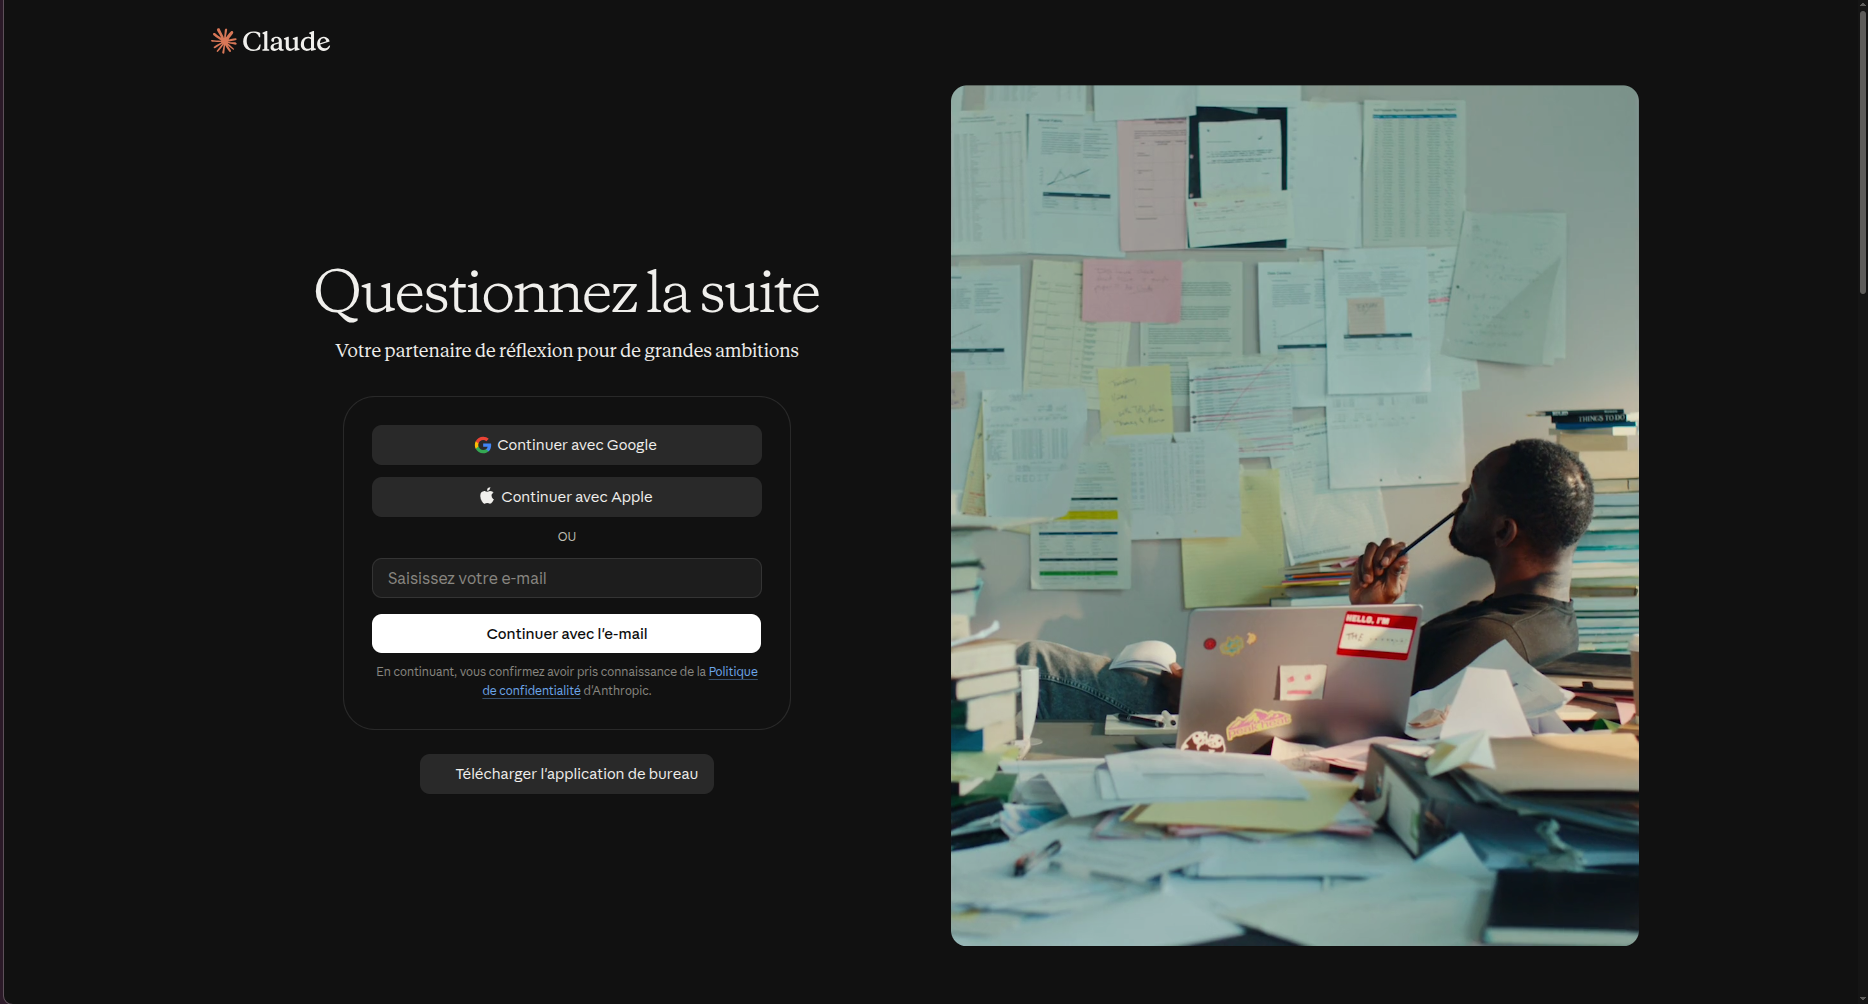
\includegraphics[width=\linewidth,height=0.75\textheight,keepaspectratio]{../images/guides/01-01_claude_ai_accueil.png}
  \caption{La page d\textquotesingle accueil de claude.ai et ses trois façons de se connecter.}
\end{figure}

\subsubsection{3.2 Les abonnements et leurs
prix}\label{32-les-abonnements-et-leurs-prix}

Un compte gratuit existe, mais un \textbf{abonnement payant} est
nécessaire pour un vrai projet : il donne beaucoup plus
d\textquotesingle usage, et il est \textbf{indispensable pour utiliser
Claude Code} (avec, à défaut, un compte de développeur « Console »
facturé à l\textquotesingle usage).

Prix relevés sur les pages officielles le 19 septembre 2026 (en dollars
américains, hors taxes) :

\begin{longtable}[]{@{}
  >{\raggedright\arraybackslash}p{(\linewidth - 4\tabcolsep) * \real{0.2050}}
  >{\raggedright\arraybackslash}p{(\linewidth - 4\tabcolsep) * \real{0.3825}}
  >{\raggedright\arraybackslash}p{(\linewidth - 4\tabcolsep) * \real{0.3825}}@{}}
\toprule\noalign{}
\begin{minipage}[b]{\linewidth}\raggedright
Abonnement
\end{minipage} & \begin{minipage}[b]{\linewidth}\raggedright
Pour qui
\end{minipage} & \begin{minipage}[b]{\linewidth}\raggedright
Prix
\end{minipage} \\
\midrule\noalign{}
\endhead
\bottomrule\noalign{}
\endlastfoot
\textbf{Gratuit} & Découvrir & 0 \$, usage limité \\
\textbf{Pro} & \textbf{Usage personnel} (étudiant, indépendant) : le
plus courant & \textbf{20 \$ par mois} (un tarif annuel, plus
avantageux, existe) \\
\textbf{Max} & Usage personnel intensif, notamment beaucoup de Claude
Code & \textbf{100 \$ par mois} (« 5x » : cinq fois
l\textquotesingle usage de Pro) ou \textbf{200 \$ par mois} (« 20x » :
vingt fois) \\
\textbf{Team} & Une \textbf{équipe} ou une petite entreprise (au moins 2
membres) & Siège standard : \textbf{25 \$ par membre et par mois} (20 \$
si facturé à l\textquotesingle année) ; siège premium : \textbf{125 \$}
(100 \$ à l\textquotesingle année) \\
\textbf{Enterprise} & Une \textbf{grande organisation} : sécurité et
administration renforcées (connexion unique, journaux
d\textquotesingle audit, etc.) & Non publics : le siège donne accès à la
plateforme, et l\textquotesingle usage est facturé à part, aux tarifs de
l\textquotesingle API. Achat en libre-service à partir de 20 sièges,
avec un commercial à partir de 50. \\
\end{longtable}

\textbf{Lequel choisir ?}

\begin{itemize}
\tightlist
\item
  \textbf{Pour ce projet, un compte Pro suffit} pour commencer. Si vous
  utilisez beaucoup Claude Code, vous atteindrez plus vite les limites
  et Max peut devenir utile.
\item
  \textbf{Team} et \textbf{Enterprise} sont pensés pour le travail en
  entreprise : partage de projets entre collègues, administration
  centralisée.
\end{itemize}

\textbf{Où voir cette page depuis votre compte ?} Cliquez sur votre
profil, en bas à gauche, puis sur \textbf{« Mettre le forfait à niveau
»}. La page propose deux onglets : \textbf{« Particuliers »} (Free, Pro
et Max) et \textbf{« Team et Enterprise »}.

% --------------------------------------------------------------------
% CAPTURE : 01-02_claude_ai_tarifs.png : Page des forfaits de Claude
% Pour mettre votre image : changez seulement le nom du fichier dans \includegraphics{...}
\begin{figure}[H]
  \centering
  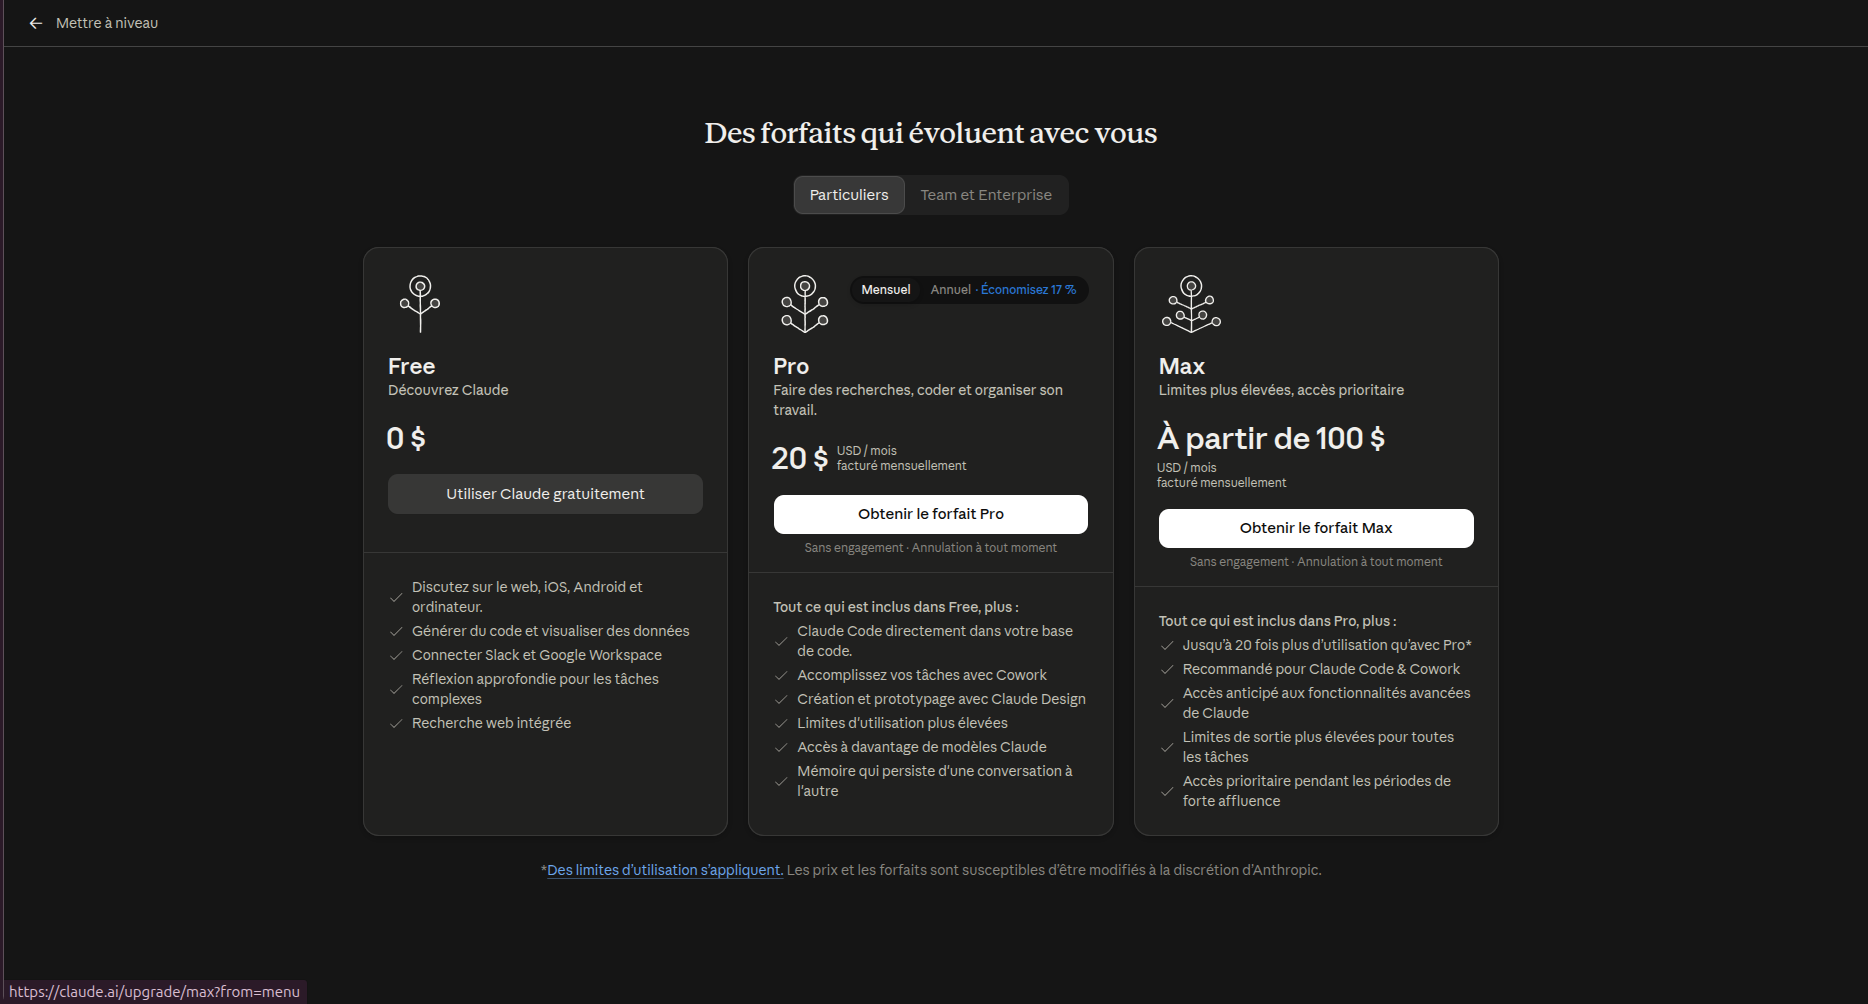
\includegraphics[width=\linewidth,height=0.75\textheight,keepaspectratio]{../images/guides/01-02_claude_ai_tarifs.png}
  \caption{La page des forfaits, onglet « Particuliers » (prix à vérifier au moment de l\textquotesingle achat).}
\end{figure}

\begin{center}\rule{0.5\linewidth}{0.5pt}\end{center}

\subsection{4. Comprendre les limites et les
sessions}\label{4-comprendre-les-limites-et-les-sessions}

C\textquotesingle est le point que les débutants comprennent le moins,
et celui qui « bloque » le plus souvent. Il faut distinguer \textbf{deux
limites} et \textbf{deux sens du mot « session »}.

\subsubsection{4.1 Les deux limites}\label{41-les-deux-limites}

\begin{longtable}[]{@{}
  >{\raggedright\arraybackslash}p{(\linewidth - 4\tabcolsep) * \real{0.1740}}
  >{\raggedright\arraybackslash}p{(\linewidth - 4\tabcolsep) * \real{0.3980}}
  >{\raggedright\arraybackslash}p{(\linewidth - 4\tabcolsep) * \real{0.3980}}@{}}
\toprule\noalign{}
\begin{minipage}[b]{\linewidth}\raggedright
Limite
\end{minipage} & \begin{minipage}[b]{\linewidth}\raggedright
Ce qu\textquotesingle elle mesure
\end{minipage} & \begin{minipage}[b]{\linewidth}\raggedright
Ce qui se passe quand on l\textquotesingle atteint
\end{minipage} \\
\midrule\noalign{}
\endhead
\bottomrule\noalign{}
\endlastfoot
\textbf{Limite d\textquotesingle usage} & Le « budget de conversation »
sur une période : combien vous avez interagi avec Claude (sur claude.ai,
dans Claude Code, dans l\textquotesingle application de bureau) & Il
faut attendre la remise à zéro \\
\textbf{Limite de longueur} & La taille de la « mémoire de travail » de
Claude dans \textbf{une même conversation} (sa fenêtre de contexte) & Il
faut ouvrir une nouvelle conversation, ou laisser Claude résumer les
échanges anciens \\
\end{longtable}

\subsubsection{4.2 La « session d\textquotesingle usage » de 5
heures}\label{42-la--session-dusage--de-5-heures}

Sur les abonnements Pro et Max, l\textquotesingle usage se mesure par
\textbf{sessions} :

\begin{itemize}
\tightlist
\item
  \textbf{toutes les cinq heures}, votre limite de session est
  \textbf{remise à zéro} ;
\item
  en plus, il existe une \textbf{limite hebdomadaire}, qui
  s\textquotesingle applique à l\textquotesingle ensemble des modèles ;
\item
  ce qui compte n\textquotesingle est pas le nombre de messages mais
  leur « poids » : la longueur du message, les fichiers joints, la
  complexité de la réponse.
\end{itemize}

\textbf{Ce qui consomme le plus :} les conversations très longues, les
nombreuses pièces jointes, la réflexion étendue,
l\textquotesingle effort élevé, les connecteurs et la recherche sur le
web. Claude Code, qui lit beaucoup de fichiers, consomme aussi vite.

\subsubsection{4.3 Où surveiller sa
consommation}\label{43-ouxf9-surveiller-sa-consommation}

\begin{enumerate}
\def\labelenumi{\arabic{enumi}.}
\tightlist
\item
  Cliquez sur \textbf{votre profil, en bas à gauche} de claude.ai :
  c\textquotesingle est le bouton qui affiche votre prénom et votre
  forfait (par exemple « Hendrix · Pro »). Un menu
  s\textquotesingle ouvre.
\item
  Dans ce menu, cliquez sur \textbf{« Paramètres »} (raccourci :
  \texttt{Ctrl} + \texttt{Maj} + \texttt{,}).
\item
  Dans la colonne de gauche de la fenêtre qui s\textquotesingle ouvre,
  cliquez sur \textbf{« Utilisation »}.
\item
  Lisez les trois blocs de la page :

  \begin{itemize}
  \tightlist
  \item
    \textbf{« Session actuelle »} : une barre indique la part déjà
    utilisée (par exemple « 63 \% utilisés ») et le temps avant la
    remise à zéro (par exemple « Réinitialisation dans 2 h 16 min ») ;
  \item
    \textbf{« Limites hebdomadaires »}, ligne \textbf{« Tous les modèles
    »} : la même chose pour la semaine, avec le jour et
    l\textquotesingle heure de la remise à zéro ;
  \item
    \textbf{« Crédits d\textquotesingle utilisation »} : un interrupteur
    pour continuer à utiliser Claude quand la limite du forfait est
    atteinte. Des frais peuvent s\textquotesingle appliquer : laissez-le
    désactivé tant que vous n\textquotesingle avez pas vérifié.
  \end{itemize}
\item
  La ligne \textbf{« Dernière mise à jour »} indique quand ces chiffres
  ont été rafraîchis ; le petit bouton rond à côté les met à jour.
\end{enumerate}

% --------------------------------------------------------------------
% CAPTURE : 01-03_menu_profil.png : Menu du profil, en bas à gauche
% Pour mettre votre image : changez seulement le nom du fichier dans \includegraphics{...}
\begin{figure}[H]
  \centering
  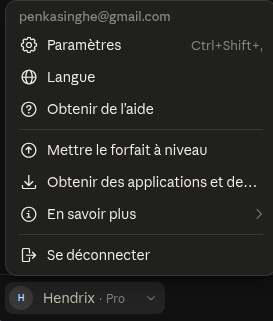
\includegraphics[width=2.84in,height=0.75\textheight,keepaspectratio]{../images/guides/01-03_menu_profil.png}
  \caption{Le menu du profil : l\textquotesingle entrée « Paramètres » ouvre la fenêtre des réglages.}
\end{figure}

% --------------------------------------------------------------------
% CAPTURE : 01-04_parametres_utilisation.png : Page Paramètres, onglet Utilisation
% Pour mettre votre image : changez seulement le nom du fichier dans \includegraphics{...}
\begin{figure}[H]
  \centering
  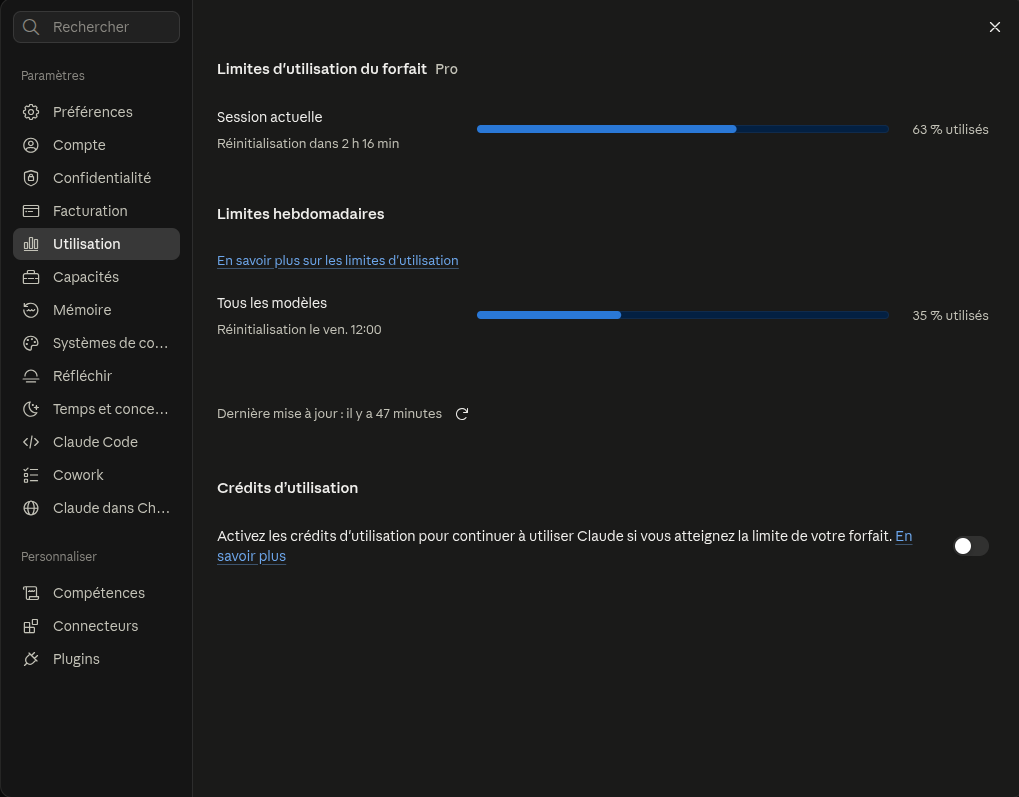
\includegraphics[width=\linewidth,height=0.75\textheight,keepaspectratio]{../images/guides/01-04_parametres_utilisation.png}
  \caption{L\textquotesingle onglet « Utilisation » : session actuelle et limites hebdomadaires.}
\end{figure}

\subsubsection{4.4 Comment consommer
moins}\label{44-comment-consommer-moins}

\begin{itemize}
\tightlist
\item
  \textbf{Une conversation par sujet.} Une conversation qui
  s\textquotesingle allonge coûte de plus en plus cher : ouvrez-en une
  nouvelle quand vous changez de sujet.
\item
  \textbf{Utilisez le mode Projet} (section 6) : les documents y sont
  chargés une fois, sans les rejoindre à chaque message.
\item
  \textbf{Retirez les fichiers inutiles} d\textquotesingle un projet.
\item
  \textbf{Coupez les options non nécessaires} : réflexion étendue,
  recherche web, connecteurs.
\item
  \textbf{Demandez des choses précises} plutôt que de faire refaire
  plusieurs fois le même travail.
\end{itemize}

\subsubsection{4.5 Le deuxième sens de « session » : la session de
travail}\label{45-le-deuxiuxe8me-sens-de--session---la-session-de-travail}

Au-delà de la limite technique, on parle de \textbf{session de travail}
: un moment de travail suivi (une demi-journée, par exemple) sur un
objectif. C\textquotesingle est une notion de \textbf{méthode},
expliquée dans le guide 2 :

\begin{quote}
\textbf{Les produits d\textquotesingle une session sont les entrées de
la session suivante.} À la fin d\textquotesingle une session, on demande
à Claude de produire un document de reprise (ce qui a été fait, décidé,
ce qui reste). Ce document est déposé dans le projet et sert de point de
départ à la session suivante.
\end{quote}

\begin{center}\rule{0.5\linewidth}{0.5pt}\end{center}

\subsection{5. Utiliser Claude dans le navigateur
(claude.ai)}\label{5-utiliser-claude-dans-le-navigateur-claudeai}

\subsubsection{5.1 Une première
conversation}\label{51-une-premiuxe8re-conversation}

\begin{enumerate}
\def\labelenumi{\arabic{enumi}.}
\tightlist
\item
  Sur claude.ai, cliquez sur le bouton \textbf{« + Nouveau »}, en haut
  de la colonne de gauche.
\item
  Cliquez dans la zone de saisie (« Comment puis-je vous aider
  aujourd\textquotesingle hui ? » sur l\textquotesingle écran
  d\textquotesingle accueil, « Écrivez un message\ldots{} » dans une
  conversation) et tapez votre demande.
\item
  Appuyez sur \texttt{Entrée} pour l\textquotesingle envoyer.
  \texttt{Maj} + \texttt{Entrée} passe à la ligne sans envoyer.
\item
  Pour \textbf{joindre un fichier} : cliquez sur le bouton \textbf{« +
  »} à gauche de la zone de saisie, puis sur \textbf{« Ajouter des
  fichiers ou des photos »} (raccourci \texttt{Ctrl} + \texttt{U}), et
  choisissez le fichier (PDF, texte, image, tableau) dans la fenêtre qui
  s\textquotesingle ouvre.
\end{enumerate}

Sur l\textquotesingle écran d\textquotesingle accueil, deux repères
utiles : le sélecteur \textbf{« Chat / Cowork »} sous la zone de saisie
(restez sur \textbf{« Chat »}) et, plus bas, la liste de vos
conversations passées : \textbf{« Épinglés »} puis \textbf{« Récents »}.
À droite de la zone de saisie, le nom du modèle est suivi
d\textquotesingle un niveau (par exemple « Sonnet 5 Élevé »).

% --------------------------------------------------------------------
% CAPTURE : 01-05_nouveau_chat.png : Le bouton Nouveau
% Pour mettre votre image : changez seulement le nom du fichier dans \includegraphics{...}
\begin{figure}[H]
  \centering
  
\includegraphics[width=1.51in,height=0.75\textheight,keepaspectratio]{../images/guides/01-05_nouveau_chat.png}
  \caption{Le bouton « + Nouveau » ouvre une nouvelle conversation.}
\end{figure}

% --------------------------------------------------------------------
% CAPTURE : 01-11_conversation_projet.png : L'écran d'accueil de claude.ai
% Pour mettre votre image : changez seulement le nom du fichier dans \includegraphics{...}
\begin{figure}[H]
  \centering
  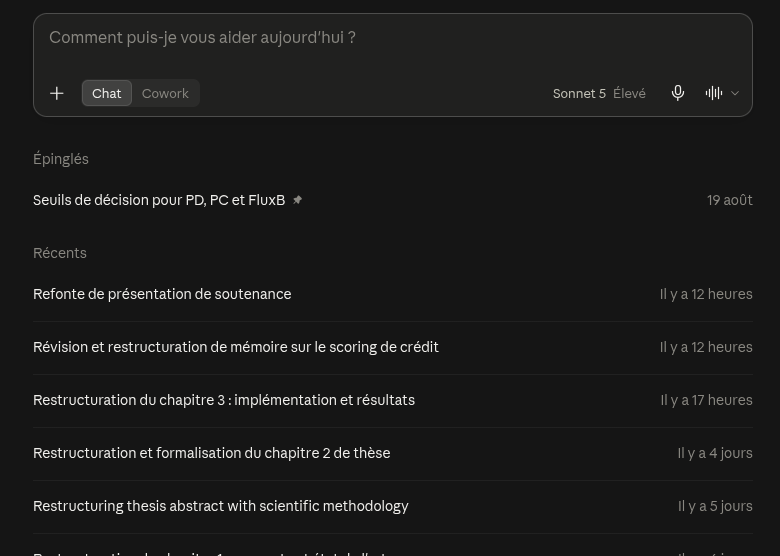
\includegraphics[width=\linewidth,height=0.75\textheight,keepaspectratio]{../images/guides/01-11_conversation_projet.png}
  \caption{L\textquotesingle écran d\textquotesingle accueil : zone de saisie, sélecteur « Chat / Cowork », modèle utilisé et conversations récentes.}
\end{figure}

\textbf{Exemples de demandes utiles :}

\begin{Verbatim}[breaklines=true,breakanywhere=true,fontsize=\small,frame=leftline,framerule=1.6pt,rulecolor=\color{credixblue},framesep=3mm,xleftmargin=2mm,xrightmargin=1mm]
Explique-moi en termes simples la différence entre un score de crédit
et une probabilité de défaut.
\end{Verbatim}

\begin{Verbatim}[breaklines=true,breakanywhere=true,fontsize=\small,frame=leftline,framerule=1.6pt,rulecolor=\color{credixblue},framesep=3mm,xleftmargin=2mm,xrightmargin=1mm]
Voici un article scientifique en PDF. Résume-le en dix lignes et dis-moi
en quoi il concerne le choix d'une méthode de sélection de variables.
\end{Verbatim}

\subsubsection{5.2 Les outils de recherche et de
réflexion}\label{52-les-outils-de-recherche-et-de-ruxe9flexion}

\begin{enumerate}
\def\labelenumi{\arabic{enumi}.}
\tightlist
\item
  Cliquez sur le bouton \textbf{« + »} à gauche de la zone de saisie. Un
  menu s\textquotesingle ouvre, avec notamment : « Ajouter des fichiers
  ou des photos », « Prendre une capture d\textquotesingle écran », «
  Ajouter au projet », « Compétences », « Connecteurs », « Système de
  design », « Ajouter des plugins », \textbf{« Recherche »} et \textbf{«
  Recherche web »}.
\item
  Cliquez sur \textbf{« Recherche web »} pour l\textquotesingle activer
  ou la désactiver : une \textbf{coche bleue} apparaît en face quand
  elle est active.
\item
  Cliquez sur \textbf{« Recherche »} pour demander une recherche
  approfondie (selon votre abonnement et votre pays, cette option peut
  varier : vérifiez dans votre menu).
\item
  Pour la réflexion, regardez à droite de la zone de saisie : le nom du
  modèle est suivi d\textquotesingle un niveau (par exemple « Sonnet 5
  Élevé »). Ce niveau règle l\textquotesingle effort de réflexion : plus
  il est haut, plus Claude réfléchit longtemps, et plus la réponse
  consomme.
\end{enumerate}

\begin{longtable}[]{@{}
  >{\raggedright\arraybackslash}p{(\linewidth - 4\tabcolsep) * \real{0.3076}}
  >{\raggedright\arraybackslash}p{(\linewidth - 4\tabcolsep) * \real{0.3312}}
  >{\raggedright\arraybackslash}p{(\linewidth - 4\tabcolsep) * \real{0.3312}}@{}}
\toprule\noalign{}
\begin{minipage}[b]{\linewidth}\raggedright
Outil
\end{minipage} & \begin{minipage}[b]{\linewidth}\raggedright
Quand l\textquotesingle utiliser
\end{minipage} & \begin{minipage}[b]{\linewidth}\raggedright
En bref
\end{minipage} \\
\midrule\noalign{}
\endhead
\bottomrule\noalign{}
\endlastfoot
\textbf{Recherche web} & Une question factuelle, une information récente
& Claude fait une ou deux recherches et répond \\
\textbf{Réflexion étendue} (niveau de réflexion du modèle) & Un
raisonnement difficile, sans besoin d\textquotesingle Internet :
mathématiques, déboguer du code, comparer des choix & Claude réfléchit
plus longtemps avant de répondre \\
\textbf{Recherche approfondie} (\emph{Research}, entrée « Recherche » du
menu) & Un vrai travail de recherche : état de l\textquotesingle art,
comparaison de méthodes & Claude enchaîne au moins cinq recherches
pendant une à trois minutes et rédige un \textbf{rapport avec des
citations} vers ses sources \\
\end{longtable}

La recherche approfondie est \textbf{très utile pour la partie «
littérature »} d\textquotesingle un projet (guide 2).

% --------------------------------------------------------------------
% CAPTURE : 01-06_outils_recherche.png : Le menu « + » de la zone de saisie
% Pour mettre votre image : changez seulement le nom du fichier dans \includegraphics{...}
\begin{figure}[H]
  \centering
  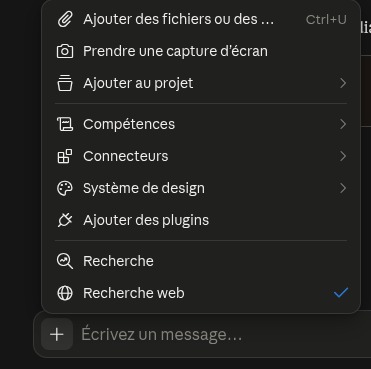
\includegraphics[width=3.86in,height=0.75\textheight,keepaspectratio]{../images/guides/01-06_outils_recherche.png}
  \caption{Le menu « + » : joindre des fichiers, ajouter au projet, « Recherche » et « Recherche web » (coche bleue quand elle est active).}
\end{figure}

\begin{quote}
\textbf{Toujours vérifier les sources.} Même avec des citations, ouvrez
les références importantes et vérifiez qu\textquotesingle elles disent
bien ce que Claude rapporte. C\textquotesingle est une règle de rigueur
pour tout travail académique.
\end{quote}

\begin{center}\rule{0.5\linewidth}{0.5pt}\end{center}

\subsection{6. Le mode Projet, indispensable pour un travail
long}\label{6-le-mode-projet-indispensable-pour-un-travail-long}

\subsubsection{6.1 Chat ou Projet ?}\label{61-chat-ou-projet-}

Un \textbf{nouveau chat} est une conversation isolée : Claude ne connaît
que ce qui s\textquotesingle y dit. Un \textbf{Projet} est un
\textbf{espace de travail} qui regroupe plusieurs conversations et des
documents partagés.

\begin{longtable}[]{@{}
  >{\raggedright\arraybackslash}p{(\linewidth - 4\tabcolsep) * \real{0.2515}}
  >{\raggedright\arraybackslash}p{(\linewidth - 4\tabcolsep) * \real{0.2395}}
  >{\raggedright\arraybackslash}p{(\linewidth - 4\tabcolsep) * \real{0.4790}}@{}}
\toprule\noalign{}
\begin{minipage}[b]{\linewidth}\raggedright
\end{minipage} & \begin{minipage}[b]{\linewidth}\raggedright
Nouveau chat
\end{minipage} & \begin{minipage}[b]{\linewidth}\raggedright
Projet
\end{minipage} \\
\midrule\noalign{}
\endhead
\bottomrule\noalign{}
\endlastfoot
Documents & À rejoindre à chaque conversation & \textbf{Chargés une
fois} dans la « base de connaissances » du projet, disponibles dans
toutes ses conversations \\
Consignes & À répéter & \textbf{Instructions du projet}, appliquées
automatiquement à chaque conversation \\
Mémoire entre conversations & Aucune & Les conversations partagent le
même contexte documentaire \\
Volume de documents & Limité à la conversation & Plus grand : sur les
abonnements payants, quand le contenu s\textquotesingle approche de la
limite, Claude passe en mode de recherche (RAG) et \textbf{peut
multiplier par 10 la capacité} \\
Travail d\textquotesingle équipe & Non & Partage possible (Team et
Enterprise) : « Peut voir » ou « Peut modifier » \\
Adapté à & Une question rapide & \textbf{Un projet qui dure plusieurs
jours ou semaines} \\
\end{longtable}

Les projets sont disponibles pour tous les comptes, y compris gratuits
(dans la limite de cinq projets).

\subsubsection{6.2 Créer un projet, pas à
pas}\label{62-cruxe9er-un-projet-pas-uxe0-pas}

\begin{enumerate}
\def\labelenumi{\arabic{enumi}.}
\tightlist
\item
  Dans la colonne de gauche de claude.ai, cliquez sur \textbf{« Projets
  »}. La page \textbf{« Projets »} s\textquotesingle ouvre : chaque
  projet y est une carte avec son nom et la date de sa dernière
  activité.
\item
  Cliquez sur le bouton \textbf{« Nouveau projet »}, en haut à droite de
  la page.
\item
  La fenêtre \textbf{« Créer un projet »} s\textquotesingle ouvre :

  \begin{itemize}
  \tightlist
  \item
    dans le champ \textbf{« Sur quoi travaillez-vous ? »} (« Nommez
    votre projet »), tapez le nom, par exemple \texttt{CREDIX} ;
  \item
    dans le champ \textbf{« Qu\textquotesingle essayez-vous de faire ?
    »}, décrivez le projet, ses objectifs, son sujet.
  \end{itemize}
\item
  Cliquez sur \textbf{« Créer un projet »} (ou sur « Annuler » pour
  abandonner).
\item
  La page du projet s\textquotesingle ouvre avec trois zones : \textbf{«
  Instructions »}, \textbf{« Contexte »} et \textbf{« Programmé »}. Les
  deux premières servent aux sections 6.3 et 6.4 ; « Programmé » (tâches
  récurrentes) ne sert pas ici.
\item
  Démarrez ensuite une conversation \textbf{à
  l\textquotesingle intérieur} du projet, avec la zone de saisie du
  projet.
\end{enumerate}

% --------------------------------------------------------------------
% CAPTURE : 01-07_liste_projets.png : Liste des projets et bouton Nouveau projet
% Pour mettre votre image : changez seulement le nom du fichier dans \includegraphics{...}
\begin{figure}[H]
  \centering
  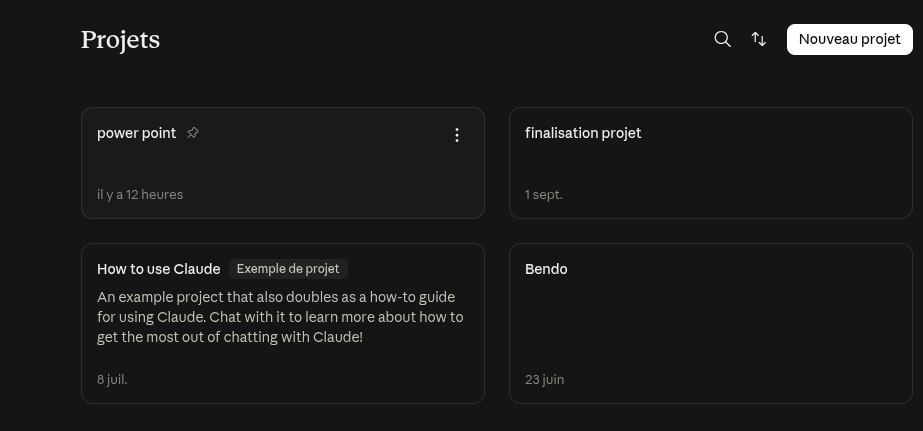
\includegraphics[width=\linewidth,height=0.75\textheight,keepaspectratio]{../images/guides/01-07_liste_projets.png}
  \caption{La page « Projets » et son bouton « Nouveau projet ».}
\end{figure}

% --------------------------------------------------------------------
% CAPTURE : 01-08_creation_projet.png : Création d'un projet : nom et description
% Pour mettre votre image : changez seulement le nom du fichier dans \includegraphics{...}
\begin{figure}[H]
  \centering
  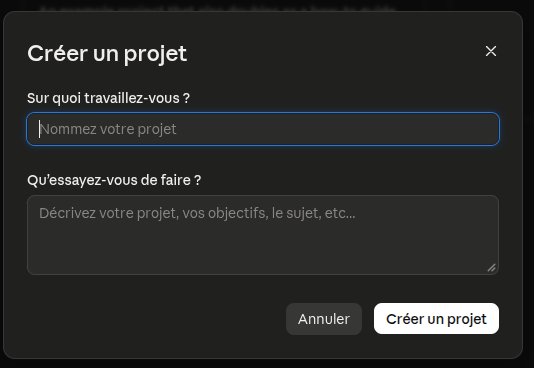
\includegraphics[width=5.56in,height=0.75\textheight,keepaspectratio]{../images/guides/01-08_creation_projet.png}
  \caption{La fenêtre « Créer un projet » : le nom, puis la description.}
\end{figure}

\subsubsection{6.3 Bien écrire les instructions du
projet}\label{63-bien-uxe9crire-les-instructions-du-projet}

Les instructions décrivent \textbf{qui est Claude dans ce projet et
comment il doit travailler}. Exemple utilisé pour CREDIX, à adapter :

\begin{Verbatim}[breaklines=true,breakanywhere=true,fontsize=\small,frame=leftline,framerule=1.6pt,rulecolor=\color{credixblue},framesep=3mm,xleftmargin=2mm,xrightmargin=1mm]
Tu es mon assistant de conception pour un mémoire d'ingénieur sur un système
de scoring de crédit.

Règles de travail :
1. Tu proposes, je décide. Avant toute décision importante, tu présentes les
   options, leurs avantages et leurs limites, puis tu attends mon accord.
2. Aucun chiffre inventé : tout chiffre vient d'un document du projet ou d'un
   calcul que je t'ai transmis. Sinon, tu dis que tu ne sais pas.
3. Tu cites tes sources (auteur, année) et tu signales quand une référence
   reste à vérifier.
4. Tu réponds en français, en termes simples, en structurant avec des titres
   et des listes.
5. À la fin de chaque session, tu produis un document de reprise en Markdown :
   ce qui a été fait, ce qui a été décidé, ce qui reste à faire.
\end{Verbatim}

\textbf{Où saisir ces instructions ?} Dans la page du projet, cliquez
sur le bouton \textbf{« + »} à droite de \textbf{« Instructions »} (le
texte grisé indique « Ajoutez des instructions pour personnaliser les
réponses de Claude »). Collez le texte, puis validez.

% --------------------------------------------------------------------
% CAPTURE : 01-09_instructions_projet.png : Panneau d'un projet neuf
% Pour mettre votre image : changez seulement le nom du fichier dans \includegraphics{...}
\begin{figure}[H]
  \centering
  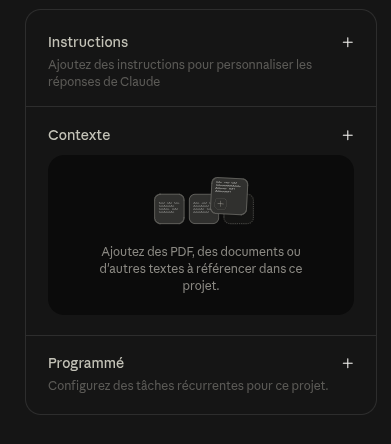
\includegraphics[width=4.07in,height=0.75\textheight,keepaspectratio]{../images/guides/01-09_instructions_projet.png}
  \caption{Le panneau d\textquotesingle un projet neuf : « Instructions », « Contexte » et « Programmé ».}
\end{figure}

\subsubsection{6.4 Que mettre dans la base de connaissances (le «
Contexte »)
?}\label{64-que-mettre-dans-la-base-de-connaissances-le--contexte--}

\begin{itemize}
\tightlist
\item
  le \textbf{cahier des charges} et les documents de conception déjà
  produits ;
\item
  les \textbf{articles scientifiques} (PDF) sur lesquels
  s\textquotesingle appuient les choix ;
\item
  les \textbf{résultats} d\textquotesingle expériences (exports,
  rapports) ;
\item
  les \textbf{documents de reprise} de chaque session précédente ;
\item
  le \textbf{journal de bord} et le \textbf{registre des décisions}
  (voir guide 2).
\end{itemize}

Pour CREDIX, la première séance de travail a justement consisté à
\textbf{faire l\textquotesingle inventaire des ressources du projet} et
à rédiger les instructions du projet, avant de poser la moindre question
de fond.

\textbf{Comment ajouter des fichiers ?} Dans la page du projet, cliquez
sur le bouton \textbf{« + »} à droite de \textbf{« Contexte »} (le texte
indique « Ajoutez des PDF, des documents ou d\textquotesingle autres
textes à référencer dans ce projet »), puis choisissez vos fichiers sur
l\textquotesingle ordinateur. Chaque fichier apparaît sous la forme
d\textquotesingle une carte avec son nom, sa taille et son type (TXT,
MD, PDF\ldots). Une \textbf{barre de capacité} indique la part déjà
utilisée (par exemple « 58 \% de la capacité du projet utilisée ») ;
quand le contenu devient volumineux, le \textbf{« Mode de recherche »}
s\textquotesingle active : Claude cherche alors les passages utiles au
lieu de tout relire.

% --------------------------------------------------------------------
% CAPTURE : 01-10_ajout_fichiers.png : Le contexte d'un projet : fichiers ajoutés et barre de capacité
% Pour mettre votre image : changez seulement le nom du fichier dans \includegraphics{...}
\begin{figure}[H]
  \centering
  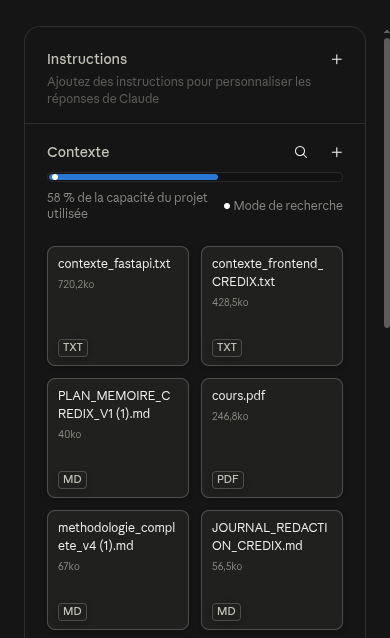
\includegraphics[width=4.06in,height=0.75\textheight,keepaspectratio]{../images/guides/01-10_ajout_fichiers.png}
  \caption{Le « Contexte » d\textquotesingle un projet : les fichiers ajoutés, la barre de capacité et le mode de recherche.}
\end{figure}

\begin{center}\rule{0.5\linewidth}{0.5pt}\end{center}

\subsection{7. Claude Code : installer et utiliser
l\textquotesingle assistant dans VS
Code}\label{7-claude-code--installer-et-utiliser-lassistant-dans-vs-code}

\subsubsection{7.1 Ce que fait Claude
Code}\label{71-ce-que-fait-claude-code}

Claude Code est l\textquotesingle assistant qui \textbf{travaille dans
votre projet} : il lit les fichiers, comprend
l\textquotesingle organisation du code, propose et effectue des
modifications, lance des commandes (tests, installation) et sait
utiliser Git. Vous lui parlez en français, comme dans claude.ai, mais
\textbf{il agit sur vos fichiers}.

\subsubsection{7.2 Ce qu\textquotesingle il faut avant
d\textquotesingle installer}\label{72-ce-quil-faut-avant-dinstaller}

\begin{itemize}
\tightlist
\item
  \textbf{VS Code, version 1.94 ou plus} (menu \emph{Aide}, puis \emph{À
  propos}, pour voir votre version) ;
\item
  un \textbf{abonnement Claude payant} (Pro, Max, Team ou Enterprise),
  ou un compte développeur « Console » : aucune clé
  d\textquotesingle API n\textquotesingle est nécessaire avec un
  abonnement.
\end{itemize}

\subsubsection{7.3 Installer l\textquotesingle extension dans VS
Code}\label{73-installer-lextension-dans-vs-code}

\begin{enumerate}
\def\labelenumi{\arabic{enumi}.}
\tightlist
\item
  Ouvrez \textbf{VS Code}.
\item
  Ouvrez la vue des \textbf{extensions} : cliquez sur
  l\textquotesingle icône des extensions dans la barre verticale de
  gauche (quatre carrés, dont un détaché), ou tapez \texttt{Ctrl} +
  \texttt{Maj} + \texttt{X} (sur Mac : \texttt{Cmd} + \texttt{Maj} +
  \texttt{X}). Le panneau \textbf{« EXTENSIONS: MARKETPLACE »}
  s\textquotesingle ouvre.
\item
  Cliquez dans la barre de recherche du panneau et tapez \textbf{claude
  code}.
\item
  Dans la liste des résultats, repérez l\textquotesingle extension
  \textbf{« Claude Code for VS Code »}. Son éditeur est
  \textbf{Anthropic}, avec un \textbf{badge bleu de vérification} à côté
  du nom. Attention : la liste contient aussi des extensions
  d\textquotesingle autres éditeurs, au nom presque identique (par
  exemple « Chat for Claude Code » ou « Claude Code Assistant for VSCode
  »). \textbf{Ne choisissez pas celles-là.}
\item
  Cliquez sur l\textquotesingle extension officielle pour ouvrir sa
  page, puis sur le bouton bleu \textbf{« Install »} (« Installer »).
\item
  Attendez la fin de l\textquotesingle installation. Si le message
  \textbf{« Restart Required »} (redémarrage requis)
  s\textquotesingle affiche à côté du nom de
  l\textquotesingle extension, redémarrez VS Code : fermez-le puis
  rouvrez-le.
\item
  Pour vérifier : l\textquotesingle extension figure dans la liste des
  extensions installées, et une \textbf{icône
  d\textquotesingle étincelle} apparaît dans VS Code (section 7.4).
\end{enumerate}

% --------------------------------------------------------------------
% CAPTURE : 01-12_vscode_recherche_extension.png : Recherche « claude code » dans les extensions de VS Code
% Pour mettre votre image : changez seulement le nom du fichier dans \includegraphics{...}
\begin{figure}[H]
  \centering
  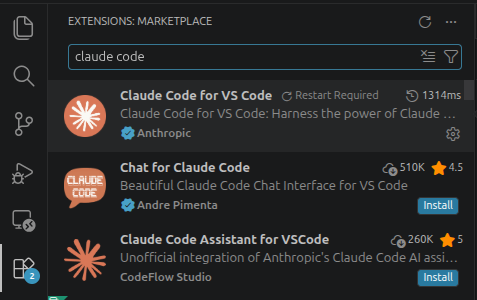
\includegraphics[width=4.97in,height=0.75\textheight,keepaspectratio]{../images/guides/01-12_vscode_recherche_extension.png}
  \caption{Recherche « claude code » : l\textquotesingle extension officielle a pour éditeur Anthropic et un badge bleu ; les autres viennent d\textquotesingle autres éditeurs.}
\end{figure}

\subsubsection{7.4 Ouvrir Claude Code et se
connecter}\label{74-ouvrir-claude-code-et-se-connecter}

\textbf{Ouvrir le panneau.} Trois façons, au choix :

\begin{enumerate}
\def\labelenumi{\arabic{enumi}.}
\tightlist
\item
  \textbf{Depuis l\textquotesingle éditeur.} Ouvrez
  d\textquotesingle abord un fichier de votre projet
  (l\textquotesingle icône n\textquotesingle apparaît que
  lorsqu\textquotesingle un fichier est ouvert), puis cliquez sur
  l\textquotesingle{}\textbf{icône d\textquotesingle étincelle}, en haut
  à droite de l\textquotesingle éditeur.
\item
  \textbf{Depuis la barre d\textquotesingle activité} (la barre
  verticale de gauche) : cliquez sur l\textquotesingle icône
  d\textquotesingle étincelle, qui ouvre la liste de vos sessions.
\item
  \textbf{Depuis la palette de commandes} : tapez \texttt{Ctrl} +
  \texttt{Maj} + \texttt{P}, écrivez « Claude Code » et choisissez
  \textbf{« Open in New Tab »} (raccourci : \texttt{Ctrl} + \texttt{Maj}
  + \texttt{Échap}).
\end{enumerate}

Le panneau \textbf{« Claude Code »} s\textquotesingle ouvre dans un
onglet de l\textquotesingle éditeur.

\textbf{Se connecter (au premier lancement seulement).}

\begin{enumerate}
\def\labelenumi{\arabic{enumi}.}
\tightlist
\item
  Le panneau vous demande de vous connecter : cliquez sur le bouton de
  connexion proposé.
\item
  Votre \textbf{navigateur} s\textquotesingle ouvre sur une page de
  claude.ai. Vérifiez que c\textquotesingle est bien le compte qui
  possède l\textquotesingle abonnement payant, puis autorisez
  l\textquotesingle accès avec le bouton de la page.
\item
  Revenez dans \textbf{VS Code} : le panneau affiche maintenant la zone
  de saisie. Vous êtes connecté.
\end{enumerate}

\textbf{Lire le panneau.} L\textquotesingle extension
s\textquotesingle affiche \textbf{en anglais}. De haut en bas : le titre
« Claude Code » ; au milieu, parfois un petit guide « Learn Claude Code
» (une liste d\textquotesingle étapes) et des messages
d\textquotesingle information, par exemple « Auto mode is enabled », que
l\textquotesingle on ferme avec la croix ; en bas, la \textbf{zone de
saisie}. Sous elle se trouvent, de gauche à droite : le bouton \textbf{«
+ »} (joindre un élément), le bouton \textbf{« / »} (commandes), le
\textbf{nom du modèle} avec son niveau d\textquotesingle effort (par
exemple « Sonnet 5 Extra high »), puis, à droite, le \textbf{mode en
cours} (par exemple « Auto ») et le \textbf{bouton
d\textquotesingle envoi} (une flèche).

% --------------------------------------------------------------------
% CAPTURE : 01-14_vscode_icone_etincelle.png : L'icône d'étincelle de Claude Code
% Pour mettre votre image : changez seulement le nom du fichier dans \includegraphics{...}
\begin{figure}[H]
  \centering
  
\includegraphics[width=2.90in,height=0.75\textheight,keepaspectratio]{../images/guides/01-14_vscode_icone_etincelle.png}
  \caption{L\textquotesingle icône d\textquotesingle étincelle, à l\textquotesingle extrémité de la barre d\textquotesingle outils de l\textquotesingle éditeur.}
\end{figure}

% --------------------------------------------------------------------
% CAPTURE : 01-15_vscode_panneau_ouvert.png : Panneau Claude Code ouvert dans VS Code
% Pour mettre votre image : changez seulement le nom du fichier dans \includegraphics{...}
\begin{figure}[H]
  \centering
  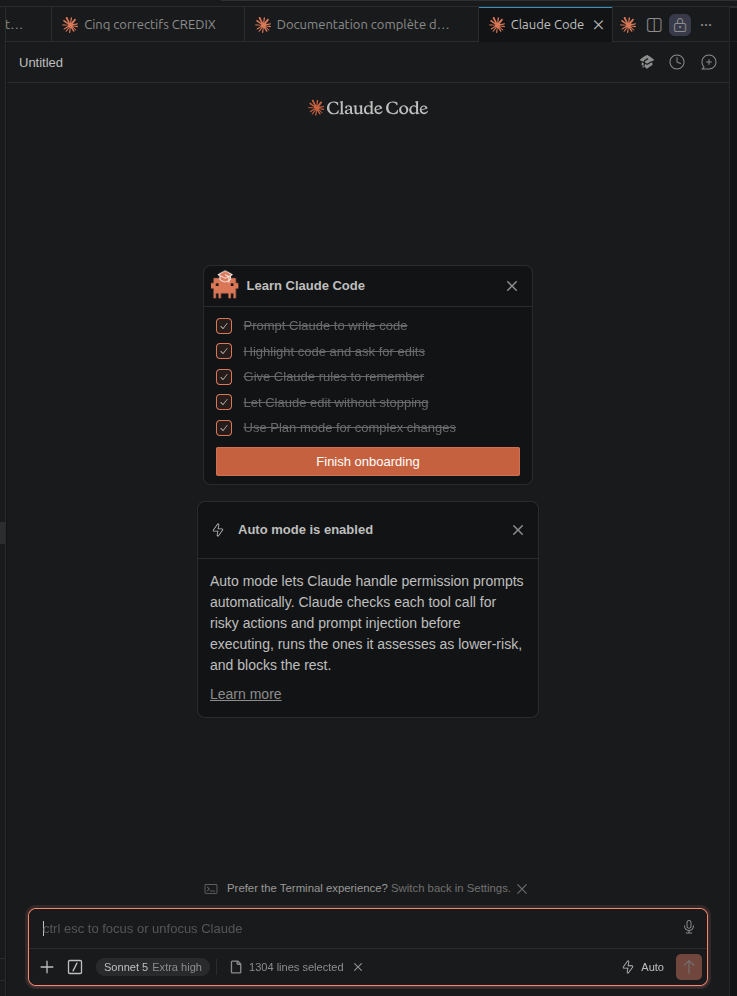
\includegraphics[width=\linewidth,height=0.75\textheight,keepaspectratio]{../images/guides/01-15_vscode_panneau_ouvert.png}
  \caption{Le panneau Claude Code : messages d\textquotesingle accueil, puis zone de saisie et réglages en bas.}
\end{figure}

\begin{quote}
\textbf{Alternative en ligne de commande.} Claude Code
s\textquotesingle installe aussi dans un terminal. Sous Linux, macOS ou
WSL :
\texttt{curl\ -fsSL\ https://claude.ai/install.sh\ \textbar{}\ bash}.
Puis \texttt{claude\ -\allowbreak{}-\allowbreak{}version} vérifie
l\textquotesingle installation, et la commande \texttt{claude}, tapée
dans le dossier d\textquotesingle un projet, démarre
l\textquotesingle assistant (connexion au premier lancement).
\end{quote}

\subsubsection{7.5 Première
utilisation}\label{75-premiuxe8re-utilisation}

\begin{enumerate}
\def\labelenumi{\arabic{enumi}.}
\tightlist
\item
  \textbf{Ouvrez le dossier de votre projet} : menu \textbf{« Fichier »}
  (\emph{File}), puis \textbf{« Ouvrir le dossier\ldots{} »} (\emph{Open
  Folder\ldots{}}) ; choisissez le dossier et validez. Son contenu
  apparaît dans la colonne de gauche de VS Code.
\item
  \textbf{Ouvrez le panneau Claude Code} en cliquant sur
  l\textquotesingle icône d\textquotesingle étincelle (section 7.4).
\item
  \textbf{Cliquez dans la zone de saisie}, en bas du panneau, et tapez
  une première question :
\end{enumerate}

\begin{Verbatim}[breaklines=true,breakanywhere=true,fontsize=\small,frame=leftline,framerule=1.6pt,rulecolor=\color{credixblue},framesep=3mm,xleftmargin=2mm,xrightmargin=1mm]
Que fait ce projet ? Explique-moi son organisation en quelques lignes.
\end{Verbatim}

\begin{enumerate}
\def\labelenumi{\arabic{enumi}.}
\setcounter{enumi}{3}
\tightlist
\item
  \textbf{Envoyez} avec la touche \texttt{Entrée}, ou avec le bouton en
  forme de flèche à droite de la zone de saisie.
\item
  \textbf{Suivez le travail de Claude} : le panneau affiche ce
  qu\textquotesingle il fait au fur et à mesure (par exemple la lecture
  de fichiers), puis sa réponse rédigée. Selon le mode choisi (section
  8), il peut vous demander une autorisation avant une action : lisez la
  demande, puis acceptez ou refusez.
\item
  \textbf{Continuez la conversation} en écrivant dans la même zone de
  saisie.
\end{enumerate}

Claude lit les fichiers dont il a besoin : vous n\textquotesingle avez
pas à les lui fournir un par un. Pour lui désigner un fichier précis,
tapez le symbole \texttt{@} suivi du début du nom du fichier, puis
choisissez-le dans la liste qui s\textquotesingle affiche.

\textbf{Quelques commandes utiles}, à taper dans la zone de saisie :

\begin{longtable}[]{@{}
  >{\raggedright\arraybackslash}p{(\linewidth - 2\tabcolsep) * \real{0.2477}}
  >{\raggedright\arraybackslash}p{(\linewidth - 2\tabcolsep) * \real{0.7223}}@{}}
\toprule\noalign{}
\begin{minipage}[b]{\linewidth}\raggedright
Commande
\end{minipage} & \begin{minipage}[b]{\linewidth}\raggedright
Effet
\end{minipage} \\
\midrule\noalign{}
\endhead
\bottomrule\noalign{}
\endlastfoot
\texttt{/help} & Affiche l\textquotesingle aide et les commandes
disponibles \\
\texttt{/clear} & Efface la conversation courante (repartir
d\textquotesingle un contexte propre) \\
\texttt{/resume} & Reprend une conversation précédente \\
\texttt{/plan} devant une demande & Fait d\textquotesingle abord un
plan, sans rien modifier (section 8) \\
\texttt{/init} & Crée automatiquement un fichier \texttt{CLAUDE.md}
décrivant le projet (voir ci-dessous) \\
\end{longtable}

\subsubsection{\texorpdfstring{7.6 Le fichier \texttt{CLAUDE.md} : la
mémoire du
projet}{7.6 Le fichier CLAUDE.md : la mémoire du projet}}\label{76-le-fichier-claudemd--la-muxe9moire-du-projet}

Chaque nouvelle conversation de Claude Code démarre « à blanc ». Pour
qu\textquotesingle il connaisse les règles de \textbf{votre} projet, on
les écrit dans un fichier \textbf{\texttt{CLAUDE.md}}, placé à la racine
du dossier : Claude le lit au début de chaque conversation.

On y met, par exemple : les commandes pour lancer et tester le projet,
les conventions de code, les décisions d\textquotesingle architecture,
les interdits (« ne jamais modifier tel dossier »). La commande
\texttt{/init} en produit une première version automatiquement, que
l\textquotesingle on complète ensuite.

\begin{center}\rule{0.5\linewidth}{0.5pt}\end{center}

\subsection{8. Les modes de Claude Code, dont le mode
Plan}\label{8-les-modes-de-claude-code-dont-le-mode-plan}

\subsubsection{8.1 Les modes de
permission}\label{81-les-modes-de-permission}

Claude Code peut lire, modifier des fichiers et lancer des commandes. Le
\textbf{mode de permission} règle ce qu\textquotesingle il peut faire
\textbf{sans vous demander}. Pour le changer :

\begin{enumerate}
\def\labelenumi{\arabic{enumi}.}
\tightlist
\item
  repérez le \textbf{nom du mode en cours}, en bas à droite de la zone
  de saisie (par exemple « Auto ») ;
\item
  cliquez dessus : la liste \textbf{« Modes »} s\textquotesingle ouvre,
  avec pour chaque mode une courte description ;
\item
  cliquez sur le mode voulu. Sous la liste, un curseur \textbf{« Effort
  »} règle l\textquotesingle effort de réflexion de Claude.
\end{enumerate}

Raccourci : \texttt{Maj} + \texttt{Tab} passe au mode suivant (dans le
terminal aussi). Dans l\textquotesingle extension, les modes
s\textquotesingle affichent \textbf{en anglais} : \emph{Manual},
\emph{Edit automatically}, \emph{Plan} et \emph{Auto}.

\begin{longtable}[]{@{}
  >{\raggedright\arraybackslash}p{(\linewidth - 4\tabcolsep) * \real{0.3445}}
  >{\raggedright\arraybackslash}p{(\linewidth - 4\tabcolsep) * \real{0.3742}}
  >{\raggedright\arraybackslash}p{(\linewidth - 4\tabcolsep) * \real{0.2513}}@{}}
\toprule\noalign{}
\begin{minipage}[b]{\linewidth}\raggedright
Mode
\end{minipage} & \begin{minipage}[b]{\linewidth}\raggedright
Ce qui s\textquotesingle exécute sans demander
\end{minipage} & \begin{minipage}[b]{\linewidth}\raggedright
Quand l\textquotesingle utiliser
\end{minipage} \\
\midrule\noalign{}
\endhead
\bottomrule\noalign{}
\endlastfoot
\textbf{Manuel} (\emph{default}) & La lecture seulement : tout le reste
demande votre accord & Travail sensible, on veut tout relire \\
\textbf{Modifier automatiquement} (\emph{acceptEdits}) & Lecture,
modification de fichiers et commandes simples (créer un dossier,
copier\ldots) & On relit le code au fur et à mesure \\
\textbf{Plan} (\emph{plan}) & Lecture seulement : Claude \textbf{explore
et propose un plan, sans rien modifier} & \textbf{Avant de changer quoi
que ce soit} \\
\textbf{Auto} (\emph{auto}) & Presque tout, avec des vérifications de
sécurité en arrière-plan & Longues tâches, moins
d\textquotesingle interruptions \\
\textbf{Contournement} (\emph{bypassPermissions}) & Tout, sans aucune
vérification & \textbf{À éviter} (réservé à des machines isolées) \\
\end{longtable}

Sur les abonnements Pro, Max et Team, le mode de départ est
\textbf{Auto}. Les libellés peuvent légèrement varier selon la version
de l\textquotesingle extension.

% --------------------------------------------------------------------
% CAPTURE : 01-18_modes_permission.png : La liste des modes
% Pour mettre votre image : changez seulement le nom du fichier dans \includegraphics{...}
\begin{figure}[H]
  \centering
  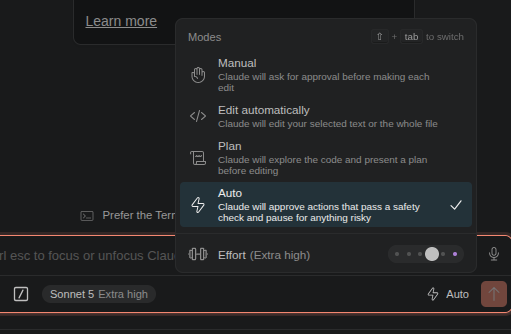
\includegraphics[width=5.32in,height=0.75\textheight,keepaspectratio]{../images/guides/01-18_modes_permission.png}
  \caption{La liste « Modes » : Manual, Edit automatically, Plan, Auto, et le curseur « Effort ».}
\end{figure}

\subsubsection{8.2 Le mode Plan : réfléchir avant
d\textquotesingle agir}\label{82-le-mode-plan--ruxe9fluxe9chir-avant-dagir}

En \textbf{mode Plan}, Claude Code \textbf{explore le projet et rédige
un plan d\textquotesingle action, mais ne modifie rien}.
C\textquotesingle est le mode à utiliser :

\begin{itemize}
\tightlist
\item
  \textbf{au début d\textquotesingle un travail} : à partir
  d\textquotesingle un document de conception, il produit la
  \textbf{liste des tâches à réaliser} (la « TODO ») ;
\item
  \textbf{avant chaque ajout ou modification} d\textquotesingle un
  module : on relit ce que Claude compte faire, on corrige, puis on
  valide.
\end{itemize}

\textbf{Pas à pas :}

\begin{enumerate}
\def\labelenumi{\arabic{enumi}.}
\tightlist
\item
  \textbf{Passez en mode Plan.} Cliquez sur le nom du mode en cours (en
  bas à droite de la zone de saisie), puis sur \textbf{« Plan »} dans la
  liste. Autres façons : taper \texttt{/plan} au début de votre demande,
  ou appuyer sur \texttt{Maj} + \texttt{Tab} jusqu\textquotesingle à ce
  que « Plan » s\textquotesingle affiche. Vérifiez que le nom du mode
  indiqué est bien \textbf{« Plan »}.
\item
  \textbf{Écrivez votre demande} dans la zone de saisie, par exemple : «
  Lis le document docs/guides/03\_conception\_MVP.md et propose un plan
  de réalisation, module par module. » Envoyez avec \texttt{Entrée}.
\item
  \textbf{Attendez.} Claude lit les fichiers et réfléchit. À ce stade,
  \textbf{aucun fichier n\textquotesingle est créé ni modifié}.
\item
  \textbf{Lisez le plan.} Il s\textquotesingle ouvre comme un
  \textbf{document Markdown} dans VS Code : un titre, des parties, une
  liste d\textquotesingle étapes. Lisez-le en entier, comme vous relirez
  un document de conception.
\item
  \textbf{Faites corriger si besoin.} Vous pouvez ajouter des
  commentaires dans le plan, à côté des passages à corriger, comme dans
  une relecture. Sinon, écrivez vos remarques dans la zone de saisie :
  Claude révise le plan.
\item
  \textbf{Approuvez quand le plan vous convient.} Trois réponses sont
  proposées :

  \begin{itemize}
  \tightlist
  \item
    \textbf{Oui, en mode Auto} : Claude passe à la réalisation avec un
    minimum d\textquotesingle interruptions ;
  \item
    \textbf{Oui, en approuvant chaque modification à la main}
    (recommandé au début) : Claude demande votre accord avant chaque
    changement ;
  \item
    \textbf{Non, continuer à planifier} : on reste en mode Plan et on
    précise ce qu\textquotesingle il faut changer.
  \end{itemize}
\item
  \textbf{Gardez le plan.} Une fois validé, il sert de \textbf{liste des
  tâches (TODO)} du projet : copiez-le dans un fichier du dossier du
  projet (guide 2, section 11.1).
\end{enumerate}

\begin{quote}
\textbf{Règle pratique.} Un travail qui touche plusieurs fichiers
commence \textbf{toujours} par un plan. C\textquotesingle est moins cher
(pas de fausses pistes) et plus sûr (vous validez avant que le code
change).
\end{quote}

\begin{center}\rule{0.5\linewidth}{0.5pt}\end{center}

\subsection{9. Bonnes pratiques et
précautions}\label{9-bonnes-pratiques-et-pruxe9cautions}

\subsubsection{9.1 Bien demander}\label{91-bien-demander}

\begin{itemize}
\tightlist
\item
  \textbf{Soyez précis.} Au lieu de « corrige le bug », écrivez : «
  corrige le bug où l\textquotesingle écran reste blanc après une erreur
  de mot de passe ».
\item
  \textbf{Procédez par étapes.} Découpez un gros travail : une base de
  données, puis les routes, puis l\textquotesingle écran.
\item
  \textbf{Faites explorer d\textquotesingle abord.} « Analyse la
  structure de la base de données » avant « ajoute un tableau de bord ».
\item
  \textbf{Parlez comme à un collègue} : décrivez
  l\textquotesingle objectif, pas seulement la tâche.
\end{itemize}

\subsubsection{9.2 Précautions}\label{92-pruxe9cautions}

\begin{itemize}
\tightlist
\item
  \textbf{Ne collez jamais de secrets} (mots de passe, clés
  d\textquotesingle API, contenu d\textquotesingle un fichier
  \texttt{.env}) dans une conversation.
\item
  \textbf{Relisez les modifications} avant de les accepter (VS Code
  montre les différences ligne par ligne).
\item
  \textbf{Travaillez sous Git} : chaque étape validée est enregistrée,
  on peut revenir en arrière.
\item
  \textbf{Vérifiez ce qui compte} : chiffres, références, résultats de
  tests. Claude peut se tromper, y compris avec assurance.
\item
  \textbf{Données réelles de clients} : ne les confiez pas à un outil
  externe sans autorisation. CREDIX a été conçu sur un jeu de données
  public pour cette raison.
\end{itemize}

\begin{center}\rule{0.5\linewidth}{0.5pt}\end{center}

\subsection{10. Glossaire et sources
officielles}\label{10-glossaire-et-sources-officielles}

\subsubsection{10.1 Glossaire}\label{101-glossaire}

\begin{longtable}[]{@{}
  >{\raggedright\arraybackslash}p{(\linewidth - 2\tabcolsep) * \real{0.2515}}
  >{\raggedright\arraybackslash}p{(\linewidth - 2\tabcolsep) * \real{0.7185}}@{}}
\toprule\noalign{}
\begin{minipage}[b]{\linewidth}\raggedright
Terme
\end{minipage} & \begin{minipage}[b]{\linewidth}\raggedright
Explication simple
\end{minipage} \\
\midrule\noalign{}
\endhead
\bottomrule\noalign{}
\endlastfoot
\textbf{Anthropic} & L\textquotesingle entreprise qui développe
Claude \\
\textbf{Abonnement} & Formule payante (Pro, Max, Team, Enterprise) qui
donne accès à plus d\textquotesingle usage \\
\textbf{Session (d\textquotesingle usage)} & Période de 5 heures au bout
de laquelle la limite de session est remise à zéro \\
\textbf{Session (de travail)} & Moment de travail suivi sur un objectif,
qui se conclut par un document de reprise \\
\textbf{Contexte} & Ce que Claude « a en mémoire » dans une
conversation \\
\textbf{Projet} & Espace de travail regroupant conversations,
instructions et documents \\
\textbf{Base de connaissances} & Les documents chargés dans un projet \\
\textbf{RAG} & Technique où Claude cherche les passages utiles dans une
grande masse de documents, au lieu de tout lire \\
\textbf{Claude Code} & L\textquotesingle assistant de programmation qui
travaille dans vos dossiers \\
\textbf{Mode Plan} & Mode où Claude propose un plan sans rien
modifier \\
\textbf{CLAUDE.md} & Fichier de consignes permanentes
d\textquotesingle un projet, lu à chaque conversation \\
\textbf{Markdown (.md)} & Format de texte simple avec titres et listes ;
c\textquotesingle est le format « naturel » de Claude \\
\end{longtable}

\subsubsection{10.2 Sources officielles (consultées le 19 septembre
2026)}\label{102-sources-officielles-consultuxe9es-le-19-septembre-2026}

\begin{itemize}
\tightlist
\item
  Abonnement Pro :
  \url{https://support.claude.com/en/articles/8325606-what-is-the-pro-plan}
\item
  Abonnement Max :
  \url{https://support.claude.com/en/articles/11049741-what-is-the-max-plan}
\item
  Abonnement Team :
  \url{https://support.claude.com/en/articles/9266767-what-is-the-team-plan}
\item
  Abonnement Enterprise :
  \url{https://support.claude.com/en/articles/9797531-what-is-the-enterprise-plan}
\item
  Limites d\textquotesingle usage et de longueur :
  \url{https://support.claude.com/en/articles/11647753-how-do-usage-and-length-limits-work}
\item
  Projets :
  \url{https://support.claude.com/en/articles/9517075-what-are-projects}
\item
  Recherche web, réflexion étendue et recherche approfondie :
  \url{https://support.claude.com/en/articles/11095361-when-should-i-use-web-search-extended-thinking-and-research}
\item
  Claude Code dans VS Code :
  \url{https://code.claude.com/docs/en/vs-code}
\item
  Claude Code, démarrage rapide :
  \url{https://code.claude.com/docs/en/quickstart}
\item
  Modes de permission (dont le mode Plan) :
  \url{https://code.claude.com/docs/en/permission-modes}
\item
  Mémoire du projet (\texttt{CLAUDE.md}) :
  \url{https://code.claude.com/docs/en/memory}
\end{itemize}

\end{document}
